\begin{frame}[t]{기존 latent communication은 대체로 하나의 매체를 선택한다}
\scriptsize
\begin{center}
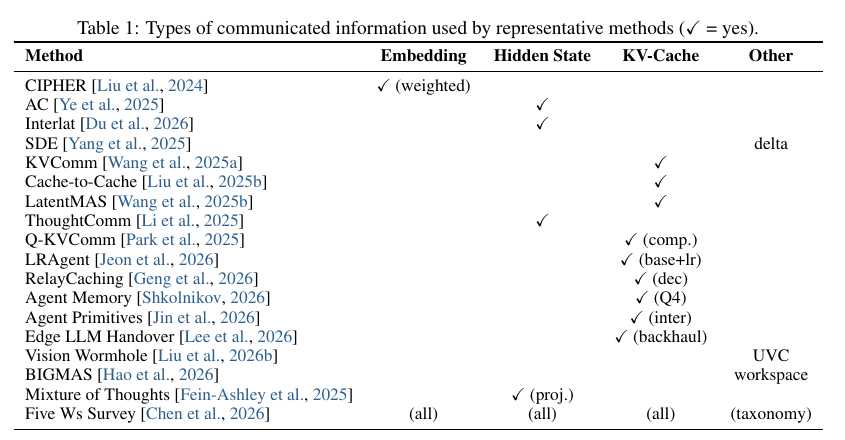
\includegraphics[width=1.02\linewidth,height=0.66\textheight,keepaspectratio]{figures/lantet_종류.png}
\end{center}

\vfill
\begin{center}
\normalsize
\fcolorbox{DeepBlue}{SoftBlue}{\parbox{0.92\linewidth}{
\centering
기존 latent communication 연구들은 모두 embedding, hidden state, KV-cache 중\\
\term{하나의 latent 매체}만 선택해 넘겨왔다.\\
\vspace{0.25em}
\textbf{그러나 이들이 정말 같은 정보인가?}
}}
\end{center}
\end{frame}

\begin{frame}[t]{Latent communication에서 넘길 수 있는 신호 종류}
\scriptsize
\begin{columns}[T,onlytextwidth]
\begin{column}{0.47\textwidth}
\begin{center}
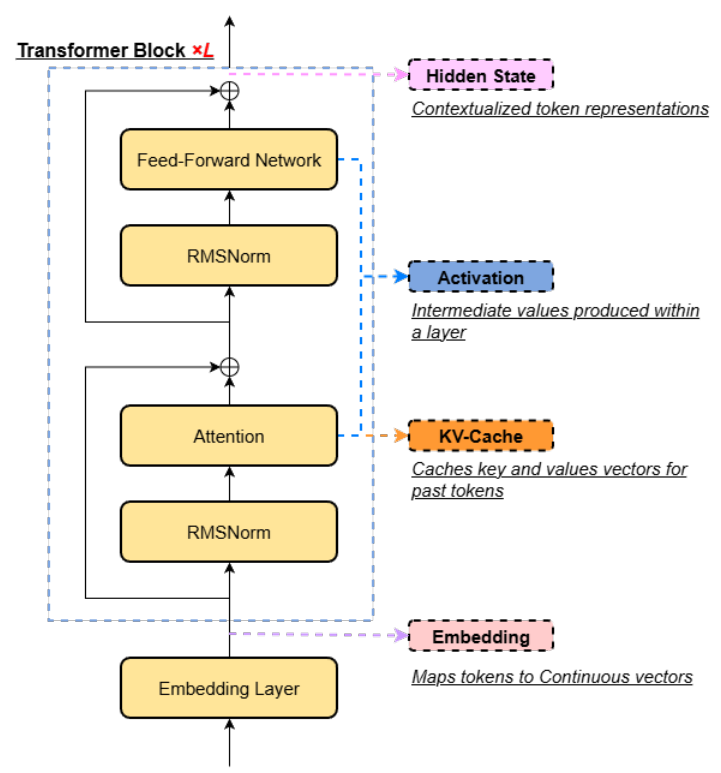
\includegraphics[width=1.06\linewidth,height=0.82\textheight,keepaspectratio]{figures/latent종류.png}
\end{center}
\end{column}
\begin{column}{0.50\textwidth}
\textbf{어떤 latent를 넘기는지에 따라 의미가 달라진다}
\vspace{0.9em}

\begin{itemize}
\setlength{\itemsep}{1.35em}
  \item \textbf{Hidden state}\\
  현재 prefix를 처리한 compact representation. belief나 intent를 압축해 전달하기 좋지만, token-level evidence memory는 약하다.

  \item \textbf{KV cache}\\
  attention에서 다시 참조할 수 있는 context memory. long evidence를 보존하지만, base memory와 role-specific signal이 섞인다.

  \item \textbf{Embedding}\\
  token이 transformer block에 들어가기 전의 lexical input representation. 원문 token identity는 강하지만,
  reasoning 이후의 belief나 attention memory는 아직 담기지 않는다.
\end{itemize}

\vspace{1.25em}
\fcolorbox{GoodGreen}{SoftGreen}{\parbox{0.92\linewidth}{
\textbf{핵심:} embedding은 입력 자체, hidden state는 compact belief, KV cache는 다시 참조 가능한 evidence memory에 가깝다.
}}
\end{column}
\end{columns}
\end{frame}

\begin{frame}[t]{왜 KV와 hidden state를 둘 다 넘기는가?}
\small
\vspace{0.7em}
\begin{columns}[T,onlytextwidth]
\begin{column}{0.46\textwidth}
\centering
\textbf{\Large KV cache}
\vspace{0.8em}

\raggedright
\begin{itemize}
  \setlength{\itemsep}{0.9em}
  \item prompt와 patient evidence를 token-level로 다시 참조할 수 있는 cache
  \item 모델의 생각이 발전하면서 어떤 evidence를 누적했는지 보존
  \item attention 과정에서 어떤 부분에 집중했는지 반영
  \item planner가 필요한 증거 위치에 다시 cross-attend할 수 있음
\end{itemize}

\vspace{0.7em}
\textbf{역할}\\
``무엇을 봤는가''를 담는\\
diagnostic evidence memory
\end{column}

\begin{column}{0.04\textwidth}
\centering
\rule{0.7pt}{0.68\textheight}
\end{column}

\begin{column}{0.46\textwidth}
\centering
\textbf{\Large Hidden state}
\vspace{0.8em}

\raggedright
\begin{itemize}
  \setlength{\itemsep}{0.9em}
  \item decode 직전 next-token prediction으로 이어지는 집약 representation
  \item 마지막 hidden state는 LM head를 거쳐 logits로 바로 변환
  \item disease posterior와 uncertainty를 compact하게 표현
  \item stop/add gate와 action policy에 직접 연결하기 쉬움
\end{itemize}

\vspace{0.7em}
\textbf{역할}\\
``현재 무엇을 믿는가''를 담는\\
diagnostic belief state
\end{column}
\end{columns}
\end{frame}

\begin{frame}[t]{구조: Dual Channel Latent Communication}
\scriptsize
\begin{center}
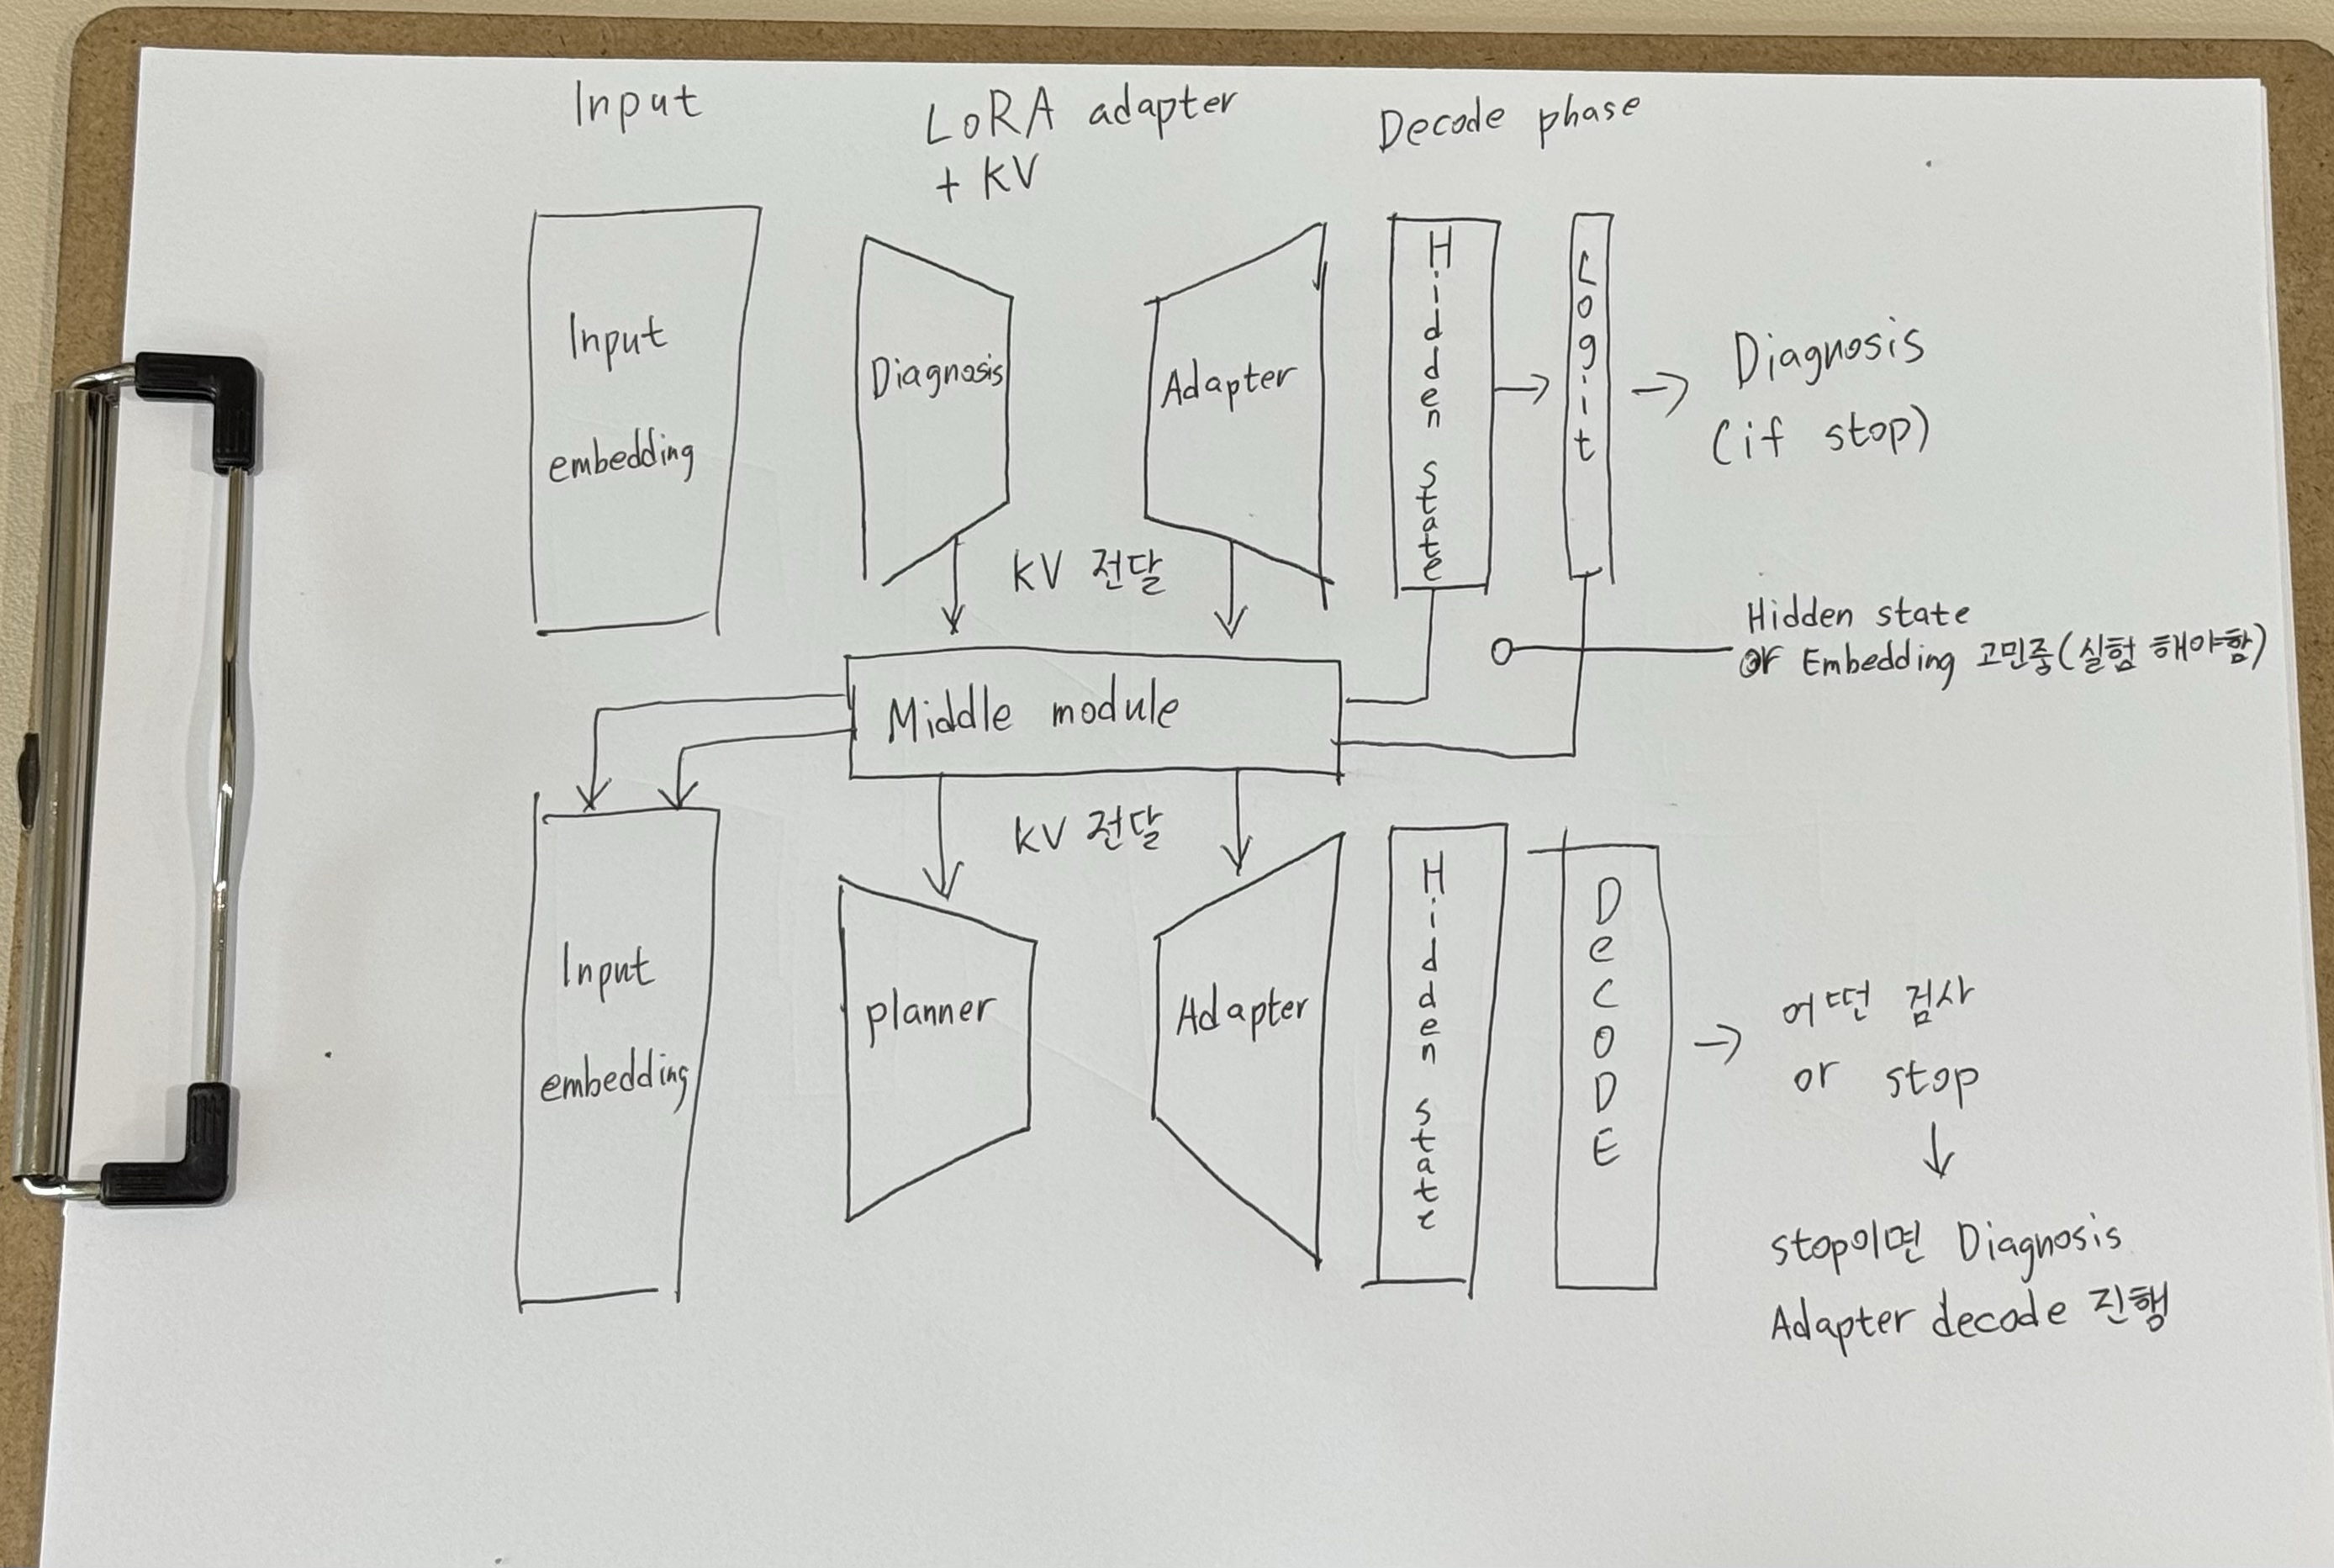
\includegraphics[width=1.06\linewidth,height=0.84\textheight,keepaspectratio]{figures/image.jpeg}
\end{center}

\end{frame}

\begin{frame}[t]{LR Agent: 멀티 LoRA adapter 세팅에서 캐시를 공유해보자}
\scriptsize
\textbf{multi-LoRA weight decomposition}
\vspace{0.15em}

\begingroup
\Large
\[
W_i = W_0 + \Delta W_i = W_0 + A_iB_i
\]
\[
Y_i = X_iW_i
    = X_iW_0 + (X_iA_i)B_i
\]
\endgroup

\vspace{0.15em}
\begin{center}
\begin{tikzpicture}[node distance=0.7cm]
\node[box, text width=0.23\linewidth] (x) {
\textbf{Input activation}\\
\(X_i\)
};
\node[box, right=0.65cm of x, text width=0.24\linewidth] (base) {
\textbf{Base cache}\\
\(X_iW_0\)
};
\node[purplebox, below=0.5cm of base, text width=0.24\linewidth] (lora) {
\textbf{LoRA cache}\\
\((X_iA_i)B_i\)
};
\node[greenbox, right=0.75cm of base, text width=0.23\linewidth] (sum) {
\textbf{Full cache}\\
\(Y_i\)
};
\draw[arrow] (x) -- (base);
\draw[arrow] (x) |- (lora);
\draw[arrow] (base) -- (sum);
\draw[arrow] (lora) -| (sum);
\end{tikzpicture}
\end{center}

\vspace{0.3em}
\textbf{KV cache에 적용하면}
\[
V_i = V_{\text{base},i} + V_{\text{adapter},i},
\quad
V_{\text{adapter},i} = (X_iA_i^V)B_i^V
\]

\begin{itemize}
  \item LR Agent는 base cache를 agent 간 공유하고, adapter output은 low-rank cache로 저장한다.
  \item 여기서 중요한 건 \term{full KV가 아니라 adapter-induced cache residual을 따로 볼 수 있다}는 점이다.
\end{itemize}
\end{frame}

\begin{frame}[t]{KV 넘기는 구조}
\scriptsize
\begin{center}
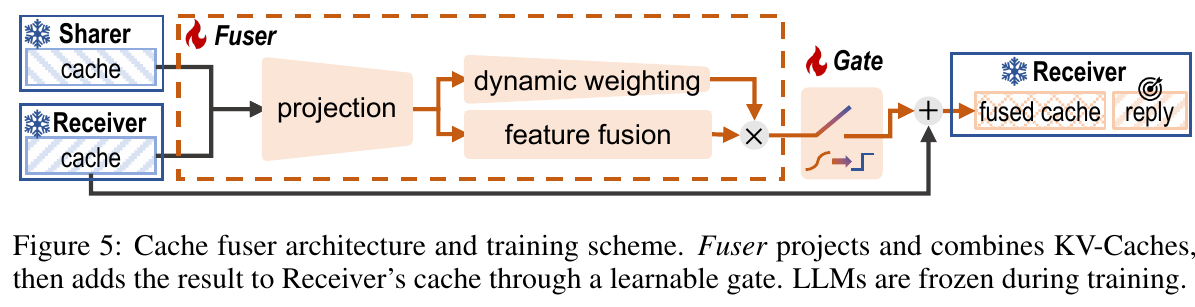
\includegraphics[width=0.94\linewidth,height=0.28\textheight,keepaspectratio]{figures/C2C.png}
\end{center}

\vspace{0.25em}
\begin{columns}[T,onlytextwidth]
\begin{column}{0.92\textwidth}
\textbf{핵심 아이디어}
\begin{itemize}
  \item Sender가 만든 \(KV_s\)를 receiver가 쓸 수 있는 \(\hat{KV}_r\)로 변환한다.
  \item 자연어 메시지 대신 latent cache를 직접 넘기므로 정보 손실과 재-prefill 비용을 줄일 수 있다.
  \item 하지만 보통 full KV를 대상으로 하므로 base memory와 role-specific adaptation이 분리되지 않는다.
\end{itemize}

\vspace{0.2em}
\textbf{우리 관점에서의 한계}
\begin{itemize}
  \item planner가 필요한 것은 전체 source context가 아니라 diagnosis adapter가 만든 diagnostic delta다.
  \item 따라서 full KV handoff보다 LoRA-induced cache만 fusion하는 편이 더 직접적이다.
\end{itemize}
\end{column}
\end{columns}
\end{frame}
